\section{Long-form games}

Thus far, we have only looked at ``single-step'' games in NFGs. Not all games can be represented by this however, with an obvious example that we have discussed being chess.

\subsection{Perfect information extensive form games}

	\begin{fdef}[Perfect Information Extensive Form Game]
		A perfect information extensive form game (PIEFG/EFG) is a $7$-tuple $\langle N,A,\mathcal{H},\mathcal{X},P,(u_i)_{i\in N}\rangle$ where
		\begin{itemize}
			\item $N$ is the set of players,
			\item $A$ is the set of all possible actions (of all players)
			\item $\mathcal{H} \subseteq \bigcup_{k=0}^{\infty} A^k$ is the set of all sequences of actions (\emph{histories}) satisfying
			\begin{itemize}
				\item $\emptyset \in \mathcal{H}$ and
				\item if $h = (a^{(0)},a^{(1)},\ldots,a^{(\tau)}) \in \mathcal{H}$, any subsequence $h' = (a^{(0)},a^{(1)},\ldots,a^{(t)})$ of $h$ (for $t \le \tau$) starting at the root is in $\mathcal{H}$,
			\end{itemize}
			\item $Z \subseteq \mathcal{H}$ is called the set of all \emph{terminal histories}, where a history $h = (a^{(0)},a^{(1)},\ldots,a^{(\tau-1)})$ is terminal if there exists no $a^{(\tau)} \in A$ with $(a^{(0)},a^{(1)},\ldots,a^{(\tau)}) \in \mathcal{H}$,
			\item $\mathcal{X} : \mathcal{H} \setminus Z \to 2^A$, called the \emph{action set selection function}, gives the set of all valid actions given a non-terminal history,
			\item $P : \mathcal{H}\setminus Z \to N$ is the \emph{player function} which gives the player who plays at a given non-terminal history, and
			\item $u_i : Z \to \R$ is the utility of player $i$.
		\end{itemize}
	\end{fdef}

	A history is essentially a path from the root in the game tree (recall our discussion of this from the first section).

	A natural next question is: what is a strategy in a PIEFG?

	\begin{fdef}[Strategy]
		A \emph{strategy} of a player in an EFG is a tuple of actions at every history where the player plays. That is, a strategy of a player $i$ is an element of
		\[ S_i = \bigtimes_{h \in \mathcal{H} : P(h) = i} \mathcal{X}(h). \]
	\end{fdef}

	We can transform EFGs to NFGs! Indeed, the above definition explicitly describes the strategy set of each player, and associated to any tuple of strategies for all the players, we can determine the payoff.\\
	This conversion has a massive explosion in size however, and equilibria in the converted NFG do not necessarily make sense in the context of the original EFG.
	% example at start of module 21

	\begin{fex}[PSNEs in PIEFGs]
		Consider the following game with two players, red and blue.
		\begin{center}
		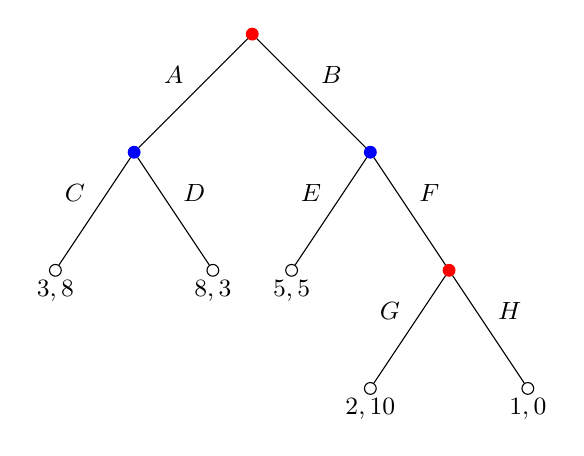
\begin{tikzpicture}
			\tikzstyle{hollow node}=[circle,draw,inner sep=1.5]
			\tikzstyle{solid node}=[circle,draw,inner sep=1.5,fill=black]
			\tikzset{
				red node/.style={circle,draw=red,fill=red,inner sep=1.5},
				blue node/.style={circle,draw=blue,fill=blue,inner sep=1.5}
			}
			\node(0)[red node]{}
				[sibling distance=30mm]
				child{node[blue node]{}
					[sibling distance=20mm]
					child{node[hollow node]{}
						node[below]{\small$3,8$}
						edge from parent node[above left]{\small$C$}}
					child{node[hollow node]{}
						node[below]{\small$8,3$}
						edge from parent node[above right]{\small$D$}}
					edge from parent node[above left]{\small$A$}}
				child{node[blue node]{}
					[sibling distance=20mm]
					child{node[hollow node]{}
						node[below]{\small$5,5$}
						edge from parent node[above left]{\small$E$}}
					child{node[red node]{}
						child{node[hollow node]{}
							node[below]{\small$2,10$}
							edge from parent node[above left]{\small$G$}}
						child{node[hollow node]{}
							node[below]{\small$1,0$}
							edge from parent node[above right]{\small$H$}}
						edge from parent node[above right]{\small$F$}} 
					edge from parent node[above right]{\small$B$}};
		\end{tikzpicture}
		\end{center}
		At the node BF, red has no reason to play $H$ since choosing $G$ results in a higher payoff. However, it is still seen that $(AH,CF)$ (at each node, the player chooses whichever of these actions is available) is a PSNE!\\
		This is a consequence of the fact that this strategy profile never even reaches the node where red chooses $G$ or $H$, so it never comes into play.
	\end{fex}

	Henceforth, we talk about PSNEs of EFGs as PSNEs of their NFG conversion.

	\begin{fdef}
		A \emph{subgame} of a game is the restriction of the game to the descendants of a history.
	\end{fdef}

	The idea behind an equilibrium should be \emph{subgame perfection}, where each player chooses the best possible action at each subgame where they play.

	\begin{fdef}[Subgame Perfect Nash Equilibrium]
		A \emph{subgame perfect nash equilibrium} (SPNE) of an EFG $G$ is a strategy profile $s \in S$ such that for any subgame $G'$ of $G$, the restriction of $s$ to $G'$ is a PSNE of $G'$.
	\end{fdef}

	Similar to MSNEs, SPNEs are guaranteed to exist in finite PIEFGs.
	Observe that any SPNE is a PSNE. As we shall now see, the algorithm to find an SPNE is quite simple.\\

	\begin{algorithm}[H]
		\DontPrintSemicolon
		\SetNoFillComment
		\SetKwProg{Fn}{}{}{}
		\SetKwFunction{backind}{{backInd}}
		\KwIn{An EFG $G$}
		\KwOut{The utility and action to be taken by a given player at a certain history}
		\Fn{\backind{history $h$}} { 
			\If{$h\in Z$} {
				\Return{$u(h),\emptyset$}\;
			}
			$\mathsf{bestUtil}_{P(h)} \gets -\infty$\;
			\ForEach{$a \in \mathcal{X}(h)$} {
				$\mathsf{utilAtChild}_{P(h)} \gets \backind{$(h,a)$}$\;
				\If{$\mathsf{utilAtChild}_{P(h)} > \mathsf{bestUtil}_{P(h)}$} {
					$\mathsf{bestUtil}_{P(h)} \gets \mathsf{utilAtChild}_{P(h)}$\;
					$\mathsf{bestAction}_{P(h)} \gets a$\;
				}
			}
			\Return{$\mathsf{bestUtil}_{P(h)},\mathsf{bestAction}_{P(h)}$}
		}
		\caption{Backward induction to determine SPNEs}
	\end{algorithm}

	The idea of subgame perfection is intrinsically tied to the above algorithm.\\
	The issue however is that we are essentially parsing the entire tree, so the algorithm is computationally very expensive. Further, some criticize the idea of SPNEs for assuming that the cognitive limit of the players is infinite (which is not realistic).\\
	It is easy to find an SPNE in simple games such as tic-tac-toe.\\

	\begin{fex}[Centipede game]
		Players $1$ and $2$ alternate, and each can play a move from $\{\mathsf{take},\mathsf{push}\}$, with a maximum of $N$ rounds, say. The game terminates when $\mathsf{take}$ is played for the first time or the limit of $N$ rounds if $\mathsf{take}$ is never played.\\
		The game also fixes some quantities $m_0,m_1$ with $m_0 > m_1$. Suppose that the game ends on round $t \in \{0,\ldots,N-1\}$ with player $p$ making the final move; let $p'$ be the other player. Then, the payoffs for the two players are as follows:
		\begin{itemize}
			\item if $p$ played $\mathsf{take}$, then $p,p'$ have payoffs of $2^t m_0$ and $2^tm_1$ respectively.
			\item if $p$ played $\mathsf{push}$, then $p,p'$ have payoffs of $2^{t+1}m_1$ and $2^{t+1}m_0$ respectively.
		\end{itemize}
		That is, if a player plays $\mathsf{push}$, they increase the size of the pot to be won, and if they play $\mathsf{take}$, the game ends, with them getting a larger amount of money.\\
		Most players except grandmasters play for a few rounds, with some of the reasons claimed for this being altruism, the difference in computational capacity of individuals and incentive difference.
	\end{fex}

	There are some other criticisms of SPNEs as well, such as that it discusses what to do if the game reaches a certain history, but the equilibrium in earlier stages might show that we cannot actually reach this history.

\subsection{Imperfect information extensive form games}

	EFGs are perfect information systems, where every player has perfect information about all developments in the game until that round. This is not useful in many practical scenarios, such as card games. EFGs also do not allow the representation of games with simultaneous moves. For example, the neighbouring kingdom dilemma we discussed in \Cref{ex: neighbouring kingdom dilemma} depends significantly on the fact that both kingdoms move simultaneously.\\
	This can be modeled as a sequential game, where the second player does not known for certain which history the game is in. This is called an \emph{information set}. Such games where players deal with information sets instead of particular histories are called imperfect information extensive form games. When the information sets are singletons, we get back PIEFGs.

	\begin{fdef}
		An \emph{imperfect information extensive form games} (IIEFG) is an $7$-tuple $\langle N,A,\mathcal{H},\mathcal{X},P,(u_i)_{i\in N},(I_i)_{i \in N}\rangle$ where
		\begin{itemize}
			\item $\langle N,A,\mathcal{H},\mathcal{X},P,(u_i)_{i\in N}\rangle$ is a PIEFG,
			\item for every $i \in N$, $I_i = (I_i^1,I_i^2,\ldots,I_i^{k(i)})$ is a partition of $\{ h \in \mathcal{H} \setminus Z : P(h) = i \}$ with the property that $\mathcal{X}(h) = \mathcal{X}(h')$ and $P(h) = P(h') = i$ whenever there exists some $j$ such that $h,h' \in I_i^j$. The $I_i^j$s are called the \emph{information sets} of player $i$, and $I_i$ the collection of information sets of $i$.
		\end{itemize}
	\end{fdef}

	At a given information set, the player and all their available actions are the same. The player is not certain which history in the information set the game is at.\\
	Since the actions now depend on the information sets and not the histories, we denote $\mathcal{X}(I_i^j) \coloneqq \mathcal{X}(h)$ for any $h \in I_i^j$.\\
	Strategies are also defined over information sets. The strategy set of player $i \in N$ is defined by
	\[ S_i = \bigtimes_{\tilde{I} \in I_i} \mathcal{X}(\tilde{I}). \]
	With IIEFGs, NFGs can be represented using EFGs, though this is not very succinct. The representation used is typically chosen on the basis of the game we are working with.

	\subsubsection{Strategies}

		In NFGs, we had mixed strategies where we randomized over pure strategies. In EFGs, randomization can be done in several ways:
		\begin{itemize}
			\item randomize over the strategies defined at the very beginning of the game, and
			\item randomize over the actions at a given information set -- we call such a strategy a behavioral strategy. This takes advantage of all the information a player has at a certain point of time.
		\end{itemize}

		\begin{fdef}
			A \emph{behavioral strategy} of a player in an IIEFG is a function that maps each of their information sets to a probability distribution over the set of actions at that information set.
		\end{fdef}

		A couple of questions come to mind seeing this: can a player attain a higher payoff using one type of strategy? Is there any sort of equivalence between mixed and behavioral strategies.

		Given a node $x$, mixed/behavioral strategy $\sigma_i$, and a mixed/behavioral strategy vector $\xi_{-i}$, denote by $p(x;\sigma_i,\chi_{-i})$ the probability of going to the node $x$ in a game.
		\begin{fdef}[Equivalence of mixed and behavioral strategies]
			A mixed strategy $\sigma_i$ and a behavioral strategy $b_i$ of a player $i$ in an IIEFG are \emph{equivalent} if for every mixed/behavioral strategy vector $\xi_{-i}$ of the other players and every vertex $x$ in the game tree,
			\[ p(x;\sigma_i,\xi_{-i}) = p(x;b_i,\xi_{-i}). \]
		\end{fdef}

		% add example from module 24 

		Now, by definition, equivalence implies that the above equality holds at leaf nodes.\\
		In fact, it suffices to check that it holds at leaf nodes! Given an arbitrary non-leaf nodes, the probability of reaching that node is equal to the sum of the probabilities of reaching the leaf nodes in the subtree, so equality at the leaves implies equality at non-leaves.\\
		As a result, we get the following.

		\begin{ftheo}[Utility Equivalence]
			If $\sigma_i,b_i$ are equivalent, then for every mixed/behavioral strategy vector of the other players $\xi_{-i}$ and every $j \in N$,
			\[ u_j(\sigma_i,\xi_{-i}) = u_j(b_i,\xi_{-i}). \]
		\end{ftheo}
		\begin{fcor}
			Let $\sigma$ and $b$ be equivalent. Then, for all $i \in N$, $u_i(\sigma) = u_i(b)$.
		\end{fcor}

		Behavioral strategies are more natural in IIEFGs. Players plan at a given stage (i.e. information set), and don't have a master plan from the very beginning. They are also far simpler computationally, since we only need to deal with fewer variables. For example, if a player has $4$ information sets with $2$ actions each, a mixed strategy would require $2^4-1$ variables whereas a behavioral strategy requires only $4$.\\
		It turns out that behavioral strategies and mixed strategies have incomparable power, as the following two examples demonstrate. 

		\begin{fex}[There exist mixed strategies without equivalent behavioral strategies]
			\label{ex: mixed without equiv behavioral}
			Consider the following game tree with a single player.
			\begin{center}
			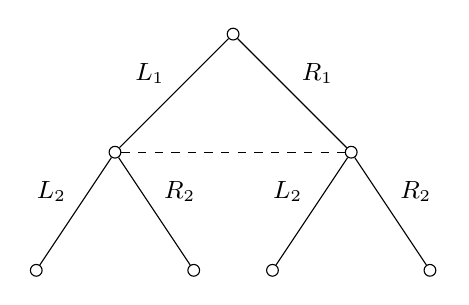
\begin{tikzpicture}
				\tikzstyle{hollow node}=[circle,draw,inner sep=1.5]
				\node(0)[hollow node]{}
					[sibling distance=30mm]
					child{node[hollow node]{}
						[sibling distance=20mm]
						child{node[hollow node]{} edge from parent node[above left]{\small$L_2$}}
						child{node[hollow node]{} edge from parent node[above right]{\small$R_2$}}
						edge from parent node[above left]{\small$L_1$}}
					child{node[hollow node]{}
						[sibling distance=20mm]
						child{node[hollow node]{} edge from parent node[above left]{\small$L_2$}}
						child{node[hollow node]{} edge from parent node[above right]{\small$R_2$}} 
						edge from parent node[above right]{\small$R_1$}};
				\draw[dashed](0-1)to(0-2);
			\end{tikzpicture}
			\end{center}
			Observe that there does not exist any behavioral strategy $b$ for the player such that $p(b;L_1R_2) = p(b;R_1L_2) = 0$. Indeed, this would require $b_1(L_2) = b_1(R_2) = 0$.\\
			On the other hand, there does exist a mixed strategy $\sigma$ that sets $\sigma(L_1R_2) = \sigma(R_1L_2) = 0$. This is easily seen on realizing that $S_1 = \{L_1,L_2\} \times \{R_1,R_2\}$, so we have complete freedom in assigning probabilities to all four leaf ndoes.
		\end{fex}

		\begin{fex}[There exist behavioral strategies without equivalent mixed strategies]
			\label{ex: behavioral without equiv mixed}
			Consider the following game tree with a single player.
			\begin{center}
			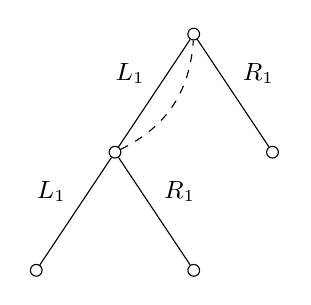
\begin{tikzpicture}
				\tikzstyle{hollow node}=[circle,draw,inner sep=1.5]
				\node(0)[hollow node]{}
					[sibling distance=20mm]
					child{node[hollow node]{}
						child{node[hollow node]{} edge from parent node[above left]{\small$L_1$}}
						child{node[hollow node]{} edge from parent node[above right]{\small$R_1$}}
						edge from parent node[above left]{\small$L_1$}}
					child{node[hollow node]{} edge from parent node[above right]{\small$R_1$}};
				\draw[dashed,bend right](0-1)to(0);
			\end{tikzpicture}
			\end{center}
			Observe that there exists no mixed strategy that goes to $L_1R_1$ with nonzero probability. Indeed, here, $S_1 = \{L_1,R_1\}$, so the path $L_1R_1$ is not even an option. \\
			On the other hand, the behavioral strategy that picks $L_1$ or $R_1$ with equal probability $1/2$ does go to $L_1R_1$ with probability $1/4$.
		\end{fex}

		In the first example above, the player remembers that they made a move but does not remember which move they made. In the second, the player does not remember that they made a move.\\

		So, when exactly does a behavioral strategy not have an equivalent mixed strategy?

		\begin{flem}
			If there exists a path from the root to some vertex $x$ that passes through the same information set twice, and if the action leading to $x$ is not the same at each of these vertices, then the player of the information set has a behavioral strategy that has no equivalent strategy.
		\end{flem}

		\begin{ftheo}
			\label{theo: behavioral has equivalent mixed}
			Consider an IIEFG such that every vertex has at least two actions. Every behavioral strategy has an equivalent mixed strategy iff each information set of a player intersects every path emanating from the root at most once.
		\end{ftheo}
		% add proof after reading msz

		When does a mixed strategy not have an equivalent mixed strategy?\\
		We need to figure out some way of formalizing the forgetfulness in \Cref{ex: mixed without equiv behavioral}.\\
		Let $X = (x_0,x_1,\ldots,x_K)$ and $\hat{X} = (x_0,\hat{x}_1,\ldots,\hat{x}_L)$ be two paths in the game tree and $I_i^j$ an information set of player $i$ that intersects the two paths are precisely one vertex, say $x_k$ and $\hat{x}_\ell$ respectively where $k<K$, $\ell<L$. Then, the two paths choose the same action at $I_i^j$ if the two actions at these vertices are identical, that is,
		\[  a_i(x_k \to x_{k+1}) = a_i(\hat{x}_\ell \to \hat{x}_{\ell+1}). \]
		In general, we also consider $a_i(x \to y)$ (where $y$ is a descendant but not necessarily a child of $x$), defined by the action $a_i(x \to x')$, where $x'$ is the child of $x$ on the path from $x$ to $y$.

		Player $i$ is said to have perfect recall if
		\begin{enumerate}
			\item any path from the root to a leaf intersects an information set of player $i$ at most once, and
			\item any two paths that end in the same information set of player $i$ pass through the same information sets of $i$ in the same order, and in every such information set, the two paths choose the same action.
		\end{enumerate}

		Let us state this more formally.

		\begin{fdef}[Perfect recall]
			Player $i$ is said to have \emph{perfect recall} if for every $I_i^j$ and pair of vertices $x,\hat{x} \in I_i^j$, if the decision vertices of $i$ are $x_i^1,x_i^2,\ldots,x_i^L = x$ and $\hat{x}_i^1,\hat{x}_i^2,\ldots,\hat{x}_i^{\hat{L}} = \hat{x}$ respectively for the two paths from the root to $x$ and $\hat{x}$, then
			\begin{enumerate}
				\item $L = \hat{L}$,
				\item for any $1 \le \ell \le L$, $x_i^\ell,\hat{x}_i^\ell \in I_i^k$ for some $k$, and
				\item for any $1 \le \ell \le L$, $a_i(x_i^\ell \to x_i^{\ell+1}) = a_i(\hat{x}_i^\ell \to \hat{x}_i^{\ell+1})$.
			\end{enumerate}
			A game is said to be of perfect recall if every player has perfect recall.
		\end{fdef}
		Why is the game in \Cref{ex: mixed without equiv behavioral} not of perfect recall?

		Observe that perfect recall subsumes the condition in \Cref{theo: behavioral has equivalent mixed}.\\
		This effectively says that ``every player remembers their choices, as well as whatever they remembered in the past''.

		Let us look at some consequences of perfect recall.\\
		Given a node $x$, let $S_i^*(x)$ be the set of pure strategies of player $i$ at which he chooses the actions leading to $x$. This is the intersections of members of $S_i$ with the paths from the root to $x$.
		\begin{ftheo}
			If $i$ is a player with perfect recall and $x,\hat{x}$ are two vertices in the same information set of $i$, then $S_i^*(x) = S_i^*(\hat{x})$.
		\end{ftheo}

		The above conclusion follows because the same information sets are seen and we take the same actions at these sets.

		\begin{ftheo}[Kuhn]
			In an IIEFG, if $i$ is a player with perfect recall, then for any mixed strategy of $i$, there exists an equivalent behavioral strategy (and vice-versa).
		\end{ftheo}
		% msz theo 6.15
		The proof is constructive in nature, with the construction using perfect recall.\\
		We remark that the converse of this theorem is \emph{not} true, as seen in \Cref{ex: behavioral without equiv mixed}.

	\subsubsection{Bayesian equilibria}

		\textcolor{red}{Henceforth, we only discuss IIEFGs with perfect recall.}
		
		What are some notions of equilibria in IIEFGs? We could extend the subgame perfection in PIEFGs, but because the histories are uncertain, we are forced to use mixed strategies. Due to the information sets, a best response cannot be defined without the ``belief'' of each player.\\
		Belief is a conditional probability distribution over the histories in an information set (where the conditioning is done over reaching the information set).

		\begin{fex*}
			Consider the following IIEFG, and the behavioral strategy described therein (by thick lines) -- in the first round, player $1$ plays $L,M,R$ with probabilities $5/12,4/12,3/12$ respectively.
			\begin{center}
			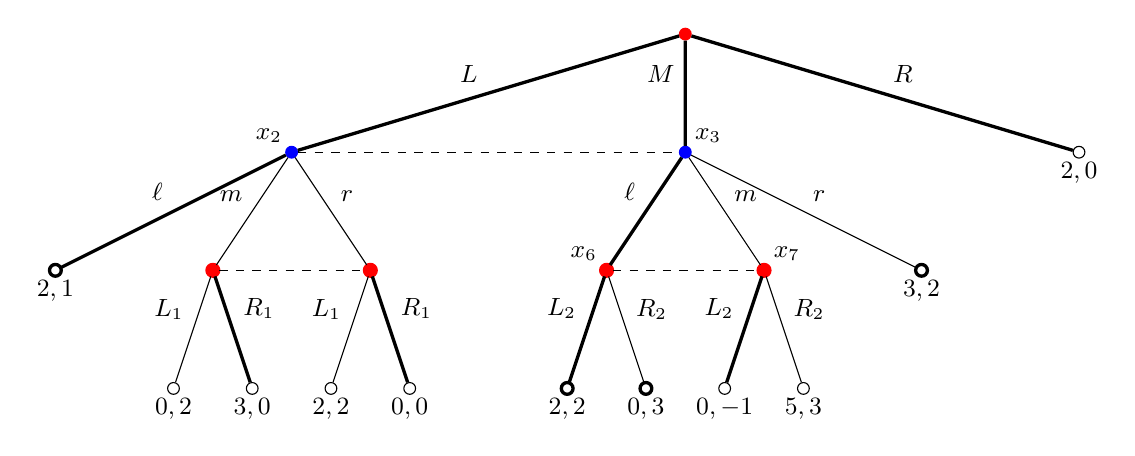
\begin{tikzpicture}
				\tikzstyle{hollow node}=[circle,draw,inner sep=1.5]
				\tikzstyle{solid node}=[circle,draw,inner sep=1.5,fill=black]
				\tikzset{
					red node/.style={circle,draw=red,fill=red,inner sep=1.5},
					blue node/.style={circle,draw=blue,fill=blue,inner sep=1.5}
				}
				\node(0)[red node]{}
					[sibling distance=50mm]
					child{node[blue node]{}
						[sibling distance=20mm]
						child{node[hollow node]{}
							node[below]{\small$2,1$}
							edge from parent[very thick] node[above left]{\small$\ell$}}
						child{node[red node]{}
							[sibling distance=10mm]
							child{node[hollow node]{}
								node[below]{\small$0,2$}
								edge from parent[thin] node[above left]{\small$L_1$}}
							child{node[hollow node]{}
								node[below]{\small$3,0$}
								edge from parent[very thick] node[above right]{\small$R_1$}}
							edge from parent[thin] node[above left]{\small$m$}}
						child{node[red node]{}
							[sibling distance=10mm]
							child{node[hollow node]{}
								node[below]{\small$2,2$}
								edge from parent[thin] node[above left]{\small$L_1$}}
							child{node[hollow node]{}
								node[below]{\small$0,0$}
								edge from parent[very thick] node[above right]{\small$R_1$}}
							edge from parent[thin] node[above right]{\small$r$}}
						child{node[]{} edge from parent[draw=none]}
						node[above left]{\small$x_2$}
						edge from parent[very thick] node[above left]{\small$L$}}
					child{node[blue node]{}
						[sibling distance=20mm]
						child{node[]{} edge from parent[draw=none]}
						child{node[red node]{}
							[sibling distance=10mm]
							child{node[hollow node]{}
								node[below]{\small$2,2$}
								edge from parent[very thick] node[above left]{\small$L_2$}}
							child{node[hollow node]{}
								node[below]{\small$0,3$}
								edge from parent[thin] node[above right]{\small$R_2$}}
							node[above left]{\small$x_6$}
							edge from parent[very thick] node[above left]{\small$\ell$}}
						child{node[red node]{}
							[sibling distance=10mm]
							child{node[hollow node]{}
								node[below]{\small$0,-1$}
								edge from parent[very thick] node[above left]{\small$L_2$}}
							child{node[hollow node]{}
								node[below]{\small$5,3$}
								edge from parent[thin] node[above right]{\small$R_2$}}
							node[above right]{\small$x_7$}
							edge from parent[thin] node[above right]{\small$m$}}
						child{node[hollow node]{}
							node[below]{\small$3,2$}
							edge from parent[thin] node[above right]{\small$r$}}
						node[above right]{\small$x_3$}
						edge from parent[very thick] node[above left]{\small$M$}}
					child{node[hollow node]{}
						node[below]{\small$2,0$}
						edge from parent[very thick] node[above right]{\small$R$}};
				\draw[dashed](0-1)to(0-2);
				\draw[dashed](0-1-2)to(0-1-3);
				\draw[dashed](0-2-2)to(0-2-3);
			\end{tikzpicture}
			\end{center}
			Now, suppose that player $2$ believes that they are at $x_6,x_7$ with probabilities $p,1-p$ respectively. If it is at $x_6$, it makes sense to choose $L_2$, and if at $x_7$, it makes sense to choose $R_2$. So, if the belief was $>2/7$ ($1-p > 2/7$), then the player chooses $R_2$. Such an action that maximizes expected utility at each information set is called \emph{sequential rationality}.\\
			
			Is the behavioral strategy described an equilibrium? Let us check this in the recursive method we did for usual SPNEs.\\
			First of all, as mentioned, we require $p \ge 5/7$.\\
			On the left subtree, the choice of $R_1$ is vacuously rational because we can never reach that subtree.\\
			Now, let the belief of player $2$ for the nodes $x_2,x_3$ be $q,1-q$ respectively. If it plays $\ell$, it gets a utility of $1$ with probability $q$ and $2$ with probability $1-q$. If it chose $m$ instead, it would get $0$ with probability $q$ and $-1$ with probability $1-q$. Finally, if it chose $r$, it would get $0$ with probability $q$ and $2$ with probability $1-q$. It is seen that the expected utility for the choice of $\ell$ is always highest. In general, we need to compare it to the expected utilities for other choices. In this case, by nature of the behavioral strategy, the belief corresponds to $q = 5/9$.\\
			Therefore, this behavioral strategy is indeed an equilibrium.\\
			This is not a unique equilibrium however. As an exercise, check whether $(MR_1R_2,m)$ is an equilibrium.
		\end{fex*}
		
		% To determine if a given mixed strategy is an equilibrium, there are a few conditions we must look at.
		% \begin{itemize}
		% 	\item Are the Bayesian beliefs consistent with $P_\sigma$? That is, is the probability that we visit 
		% 	\item 
		% \end{itemize}

		\begin{fdef}
			Let the information sets of player $i$ be $I_i = \{ I_i^k \}_{k=1}^{k(i)}$. The \emph{belief} of player $i$ is a probability distribution $\mu_i^j$ over $I_i^j$.\\
			A belief $\mu_i = \{\mu_i^j\}_{j=1}^{k(i)}$ of player $i$ is said to be a \emph{Bayesian belief} wrt the behavorial strategy $\sigma$ if it is derived from $\sigma$ using Bayes' rule. That is,
			\[ \mu_i^j(x) = \frac{P_\sigma(x)}{\sum_{y \in I_i^j} P_\sigma(y)} \]
			for all $x \in I_i^j$ and $j = 1,2,\ldots,k(i)$.\\
			A strategy $\sigma_i$ of player $i$ at information set $I_i^j$ is said to be \emph{sequentially rational} given $\sigma_{-i}$ and partial beliefs $\mu_i^j$ if
			\[ \sum_{x \in I_i^j} \mu_i^j(x) u_i(\sigma_i,\sigma_{-i} \mid x) \ge \sum_{x \in I_i^j} \mu_i^j(x) u_i(\sigma_i',\sigma_{-i} \mid x). \]
			for all actions $\sigma_i'$ at $I_i^j$.\\
			The tuple $(\sigma,\mu)$ is sequentially rational if it is sequentially rational for every player at every information set. Such a tuple $(t,\mu)$ is also called an \emph{assessment}.
		\end{fdef}

		Sequential rationality is a refinement of Nash equilibria.

		\begin{fprop}
			In a PIEFG, a behavioral strategy profile $\sigma$ is an SPNE iff the tuple $(\sigma,\hat{\mu})$ is sequentially rational.
		\end{fprop}
		Above, $\hat{\mu}$ assigns a degenerate distribution to every node.

		\begin{fdef}
			An assessment $(\sigma,\mu)$ is a \emph{perfect Bayesian equilibrium} (PBE) if for every player $i \in N$,
			\begin{enumerate}
				\item $\mu_i$ is Bayesian with respect to $\sigma$, and
				\item $\sigma_i$ is sequentially rational given $\sigma_{-i}$ and $\mu_i$.
			\end{enumerate}
		\end{fdef}
		This is often represented with only $\sigma$, because $\mu$ is obtained from $\sigma$.

	\subsubsection{Example: peer-to-peer file sharing}

		In traditional file sharing models, download rate rapidly tapers off as the number of users increases. In peer-to-peer (P2P) models however, the download rate does not change significantly with an increase in users.\\
		P2P models are very scalable and resilient to failures.
		\begin{enumerate}
			\item A \emph{protocol} is the messages that can be sent and the actions that can be taken over the network.
			\item A \emph{client} is a particular process for sending messages and taking actions.
			\item A \emph{reference client} is a specific implementation of a client.
			\item The \emph{peers} are the ones using the protocol, and are the players in the game theoretic version of this problem which we shall discuss.
		\end{enumerate}

		One of the earliest P2P systems, \emph{Napster}, had a centralized database using which users could download music form one another.\\
		Later, \emph{Gnutella} became more popular. Each peer $A$ can get a list of IP addresses of peers from a set of knwn peers (there is no server). To get a file, it broadcasts a query message to known peers, and the query response is sent by a peer $B$ who has the desired file (this response is routed back to the original requester). Finally, $A$ directly downloads the file from $B$.\\

		Now, in Gnutella, each player can choose to either share, or ``free ride'' and gain the benefits of downloading without sharing anything. A corresponding game matrix looks something like
		\begin{center}
		\begin{tabular}{|c||c|c|}
			\hline
			& \textsf{Share} & \textsf{Free} \\
			\hline\hline
			\textsf{Share} & $2,2$ & $-1,3$ \\
			\hline
			\textsf{Free} & $3,-1$ & $0,0$ \\
			\hline 
		\end{tabular}
		\end{center}

		This is very similar to the \href{ex: neighbouring kingdom dilemma}{neighbouring kingdoms dilemma} we have seen. The issue with Gnutella is that it does not take these strategic thoughts into consideration. It does in fact turn out \cite{gnutella-free-ride} that very few of the peers actually share anything.\\
		In 2005, $85\%$ (!) of the peers were free-riding. By $2013$, Gnutella comprised less than $1\%$ of worldwide P2P traffic. Many other P2P systems met the same fate.\\

		We shall look at \emph{BitTorrent}, which now comprises about $85\%$ of P2P traffic in USA. It is used for both file sharing and software distribution (like Linux).\\
		The key innovation is that it breaks files into pieces, and views it as a \emph{repeated} game, with each piece shared separately.
		\begin{enumerate}
			\item First, the user goes to a searchable directory to find a link to a \texttt{.torrent} file corresponding to the desired content.
			\item The \texttt{.torrent} file contains metadata about the content, in particular tracker URLs.
			\item The tracker provides a list of peers participating in the swarm for the content (that is, their IP address and port).
			\item The users BitTorrent client can now contact all these peers to download content.
		\end{enumerate}
		The tracker is a centralized entity that controls traffic, tracks connection between peers and their speed of upload, download etc.\\
		BitTorrent's algorithm is referred to as the \emph{optimistic unchoking} algorithm. The reference client does as follows.
		\begin{enumerate}
			\item It sets a threshold $r$ of upload speed. %This is typically the third maximum speed in recent past.
			\item If a peer $j$ uploaded to $i$ at a rate $\ge r$, unchoke $j$ in the next period.
			\item If a peer $j$ uploaded to $i$ at a rate $< r$, choke $j$ in the next period.
			\item Some peers who have just appeared may end up being choked because of this because they have not uploaded anything yet. So, every three time periods, optimistically unchoke a random peer from the neighbourhood who is currently choked, and leave them unchoked for three time periods.
		\end{enumerate}
		This is forcing a repeated game by fragmenting files. The ``leecher-seeder'' (downloader-uploader) game is a repeated version of the neighbouring kingdoms dilemma, and the strategy of the seeder is just tit-for-tat -- it cooperates as long as the leecher does as well.\\
		The reader may find a simulation of the algorithm \href{http://mg8.org/processing/bt.html}{here}.\\

		There are a couple of strategic behaviors.
		\begin{enumerate}
			\item How often should one contact the tracker?
			\item Which fragments of the file should be revealed?
			\item How many upload slots and which peers should be unchoked and at what speed?
			\item What data should others be allowed to download?
			\item Possible goals might be to minimize upload speed, maximize download speed, or perhaps some sort of balance.
		\end{enumerate}

		There are numerous attacks on BitTorrent as well, such as
		\begin{enumerate}
			\item BitThief \cite{bitthief}. The goal is to download files without uploading. It asks for peers from the tracker very frequently to grow its neighbourhood rapidly. It exploits optimistic unchoking, so never needs to upload.\\
			This can be fixed by modifying the tracker to block the IP address.
			\item Strategic Piece Revealer \cite{strategic-piece-revealer}. The reference client tells neighbours about new pieces, and requests the ``rarest'' piece first. It then tries to set up a monopoly while keeping others interested. Because we have established a monopoly over rare pieces, we can get any piece we desire. % if all adopt this, download time increases by 12%
		\end{enumerate}